\documentclass{article}

% Symbols
\usepackage{amsmath}
\usepackage{amssymb}

% Language
% \usepackage[spanish]{babel}

% Float managment
\usepackage{float}

% Color
\usepackage{xcolor}

\definecolor{dkgreen}{rgb}{0,0.6,0}
\definecolor{gray}{rgb}{0.5,0.5,0.5}
\definecolor{mauve}{rgb}{0.58,0,0.82}
\definecolor{verylightgray}{rgb}{0.92,0.92,0.92}

% Links
\usepackage{hyperref}
\hypersetup{
  colorlinks,
  urlcolor={mauve}
}

% Code-like text
\usepackage{listings}
\lstset{
  language=bash,
  aboveskip=3mm,
  belowskip=3mm,
  showstringspaces=false,
  columns=flexible,
  basicstyle={\small\ttfamily},
  numbers=none,
  extendedchars=true,
  numberstyle=\tiny\color{gray},
  keywordstyle=\color{blue},
  commentstyle=\color{dkgreen},
  stringstyle=\color{mauve},
  breaklines=true,
  breakatwhitespace=true,
  tabsize=3,
  backgroundcolor = \color{verylightgray},
}


% Margins
\usepackage{geometry}
\addtolength{\hoffset}{-0.5cm}
\addtolength{\textwidth}{1cm}
\addtolength{\voffset}{-0.5cm}
\addtolength{\textheight}{1.9cm}
\addtolength{\headsep}{0.5cm}

% Graphics
\usepackage{graphicx}

% Drawings
\usepackage{tikz}
\usetikzlibrary{arrows,shapes,matrix,decorations.pathmorphing,
                shapes.geometric,calc,babel}


% Header-Footer
\usepackage{fancyhdr}
\pagestyle{fancyplain}
\lhead{Alan Ernesto Arteaga V\'azquez \\
       Mauricio Carrasco Ruiz \\
       C\'esar Hern\'andez Cruz}
\chead{Redes de Computadoras \\ Proyecto 1}
\rhead{Fecha de entrega: \\ 25 de noviembre de 2020}

\renewcommand\headrulewidth{1.5pt}
\makeatletter
\def\headrule{
{\if@fancyplain\let\headrulewidth\plainheadrulewidth\fi
\hrule\@height\headrulewidth\@width\headwidth
\vskip 2pt% 2pt between lines
\hrule\@height.5pt\@width\headwidth% lower line w/.5pt line width
\vskip-\headrulewidth
\vskip-1.5pt}}
\makeatother

% Macros
\newcommand{\ttt}[1]{%
\texttt{#1}%
}


\begin{document}

%%%%%%%%%%%%%%%%%%%%%%%%%%%%%%%%%%%%%%%%%%%%%%%%%%%%%%%%%%%%%%%%
%%%%%%%%%%%%%%%%%%%%%%%%%%%%%%%%%%%%%%%%%%%%%%%%%%%%%%%%%%%%%%%%
%%%%%%%%%%%%%%%%%%%%%%%%%%%%%%%%%%%%%%%%%%%%%%%%%%%%%%%%%%%%%%%%
%%%%%%%%%%%%%%%%%%%%%%%%               %%%%%%%%%%%%%%%%%%%%%%%%%
%%%%%%%%%%%%%%%%%%%%%%%%%%%%%%%%%%%%%%%%%%%%%%%%%%%%%%%%%%%%%%%%
%%%%%%%%%%%%%%%%%%%%%%%%%%%%%%%%%%%%%%%%%%%%%%%%%%%%%%%%%%%%%%%%
%%%%%%%%%%%%%%%%%%%%%%%%%%%%%%%%%%%%%%%%%%%%%%%%%%%%%%%%%%%%%%%%

\section{Diagrama}

El diagrama de la configuraci\'on de nuestros
servidores se muestra en la Figura \ref{fig:diagrama}.
La componente de la derecha en el diagrama corresponde
a todos los servicios que son cubiertos por AWS.
Todos los servidores son instancias EC2; aparece en
primer lugar su nombre de dominio privado, administrado
por Route 53, despu\'es su direcci\'on IP interna (con
m\'ascara de subred 172.31.0.0), y para el servidor web
(octogatos.tech), el servidor de correo
(mail.octogatos.tech) y el NAT gateway, su direcci\'on
IP el\'astica en tercer lugar.   Como puede verse en
el diagrama, hay dos subredes p\'ublicas (una que
contiene al servidor web y al NAT gateway, y otra que
\'unicamente contiene al servidor de correo), y una
privada (que contiene a los servidores de aplicaci\'on
y de datos).   La subred p\'ublica tiene salida a
internet a trav\'es del NAT gateway, y las tres
subredes, junto con el NAT gateway, se enrutan al
internet gateway a trav\'es de la tabla de ruteo de
la VPC.

Fuera de los servicios de AWS, se utiliz\'o
\href{https://get.tech}{.tech domains} para registrar
el dominio \href{https://octogatos.tech}{octogatos.tech}.
Tambi\'en se utilizaron los servicios de DNS y CDN de
\href{https://cloudflare.com}{Cloudflare}, as\'i como
su sistema de seguridad entre el cliente y sus
servidores.

\begin{figure}[H]
  \centering
  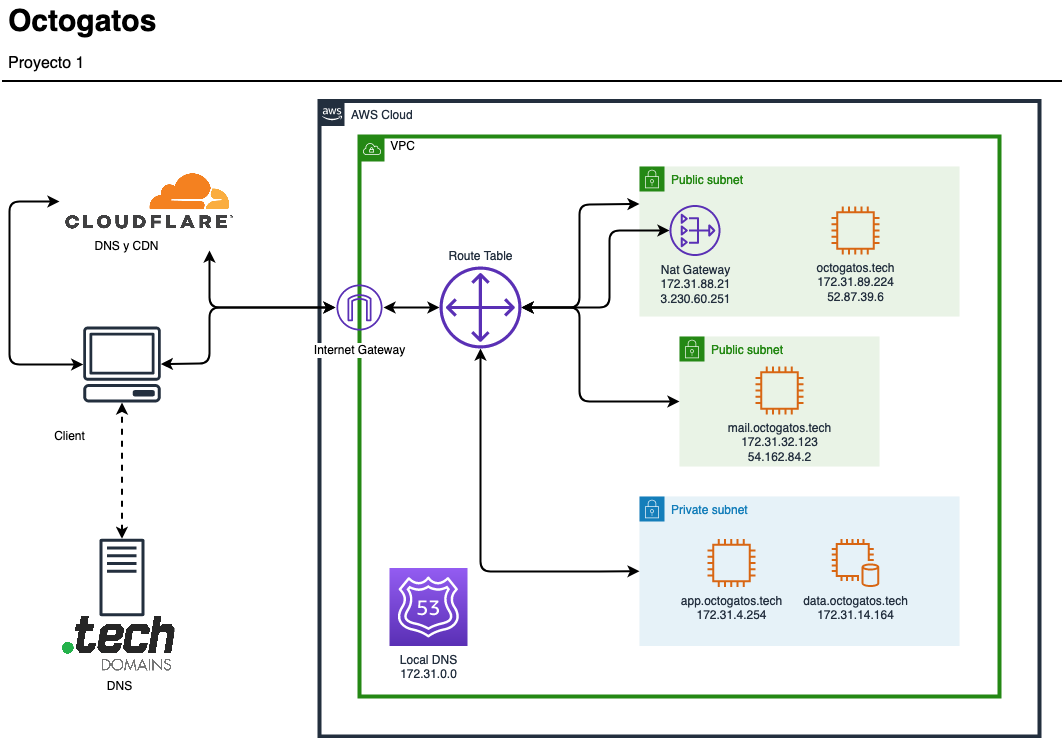
\includegraphics[width=\textwidth]{images/diagrama}
  \caption{Diagrama de configuraci\'on.}
  \label{fig:diagrama}
\end{figure}


%%%%%%%%%%%%%%%%%%%%%%%%%%%%%%%%%%%%%%%%%%%%%%%%%%%%%%%%%%%%%%%%
%%%%%%%%%%%%%%%%%%%%%%%%%%%%%%%%%%%%%%%%%%%%%%%%%%%%%%%%%%%%%%%%
%%%%%%%%%%%%%%%%%%%%%%%%%%%%%%%%%%%%%%%%%%%%%%%%%%%%%%%%%%%%%%%%
%%%%%%%%%%%%%%%%%%%%%%%%               %%%%%%%%%%%%%%%%%%%%%%%%%
%%%%%%%%%%%%%%%%%%%%%%%%%%%%%%%%%%%%%%%%%%%%%%%%%%%%%%%%%%%%%%%%
%%%%%%%%%%%%%%%%%%%%%%%%%%%%%%%%%%%%%%%%%%%%%%%%%%%%%%%%%%%%%%%%
%%%%%%%%%%%%%%%%%%%%%%%%%%%%%%%%%%%%%%%%%%%%%%%%%%%%%%%%%%%%%%%%

\section{Direcciones IPv6}

Las instancias correspondientes al servidor web y al
servidor de correo electr\'onico cuentan con direcciones
IPv6.   Para asignarle una direcci\'on IPv6 a nuestras
instancias se llevaron a cabo los siguientes pasos.
\begin{enumerate}
  \item Asociar un bloque CIDR IPv6 a nuestra VPC y
    subredes.

  \item Actualizar las tablas de enrutamiento.

  \item Actualizar los grupos de seguridad.

  \item Asignar direcciones IPv6 a las instancias.
\end{enumerate}

No ahondaremos en las instrucciones precisas para estos
pasos, pues pueden consultarse en el documento de AWS
que se encuentra en \href{https://docs.aws.amazon.com/vpc/latest/userguide/vpc-migrate-ipv6.html}{esta liga}.  Sin embargo,
creemos valioso mencionar que, aunque en el Paso 3 diga
que las reglas de ACL se configuran autom\'aticamente,
nosotros tuvimos que hacerlo a mano.

%%%%%%%%%%%%%%%%%%%%%%%%%%%%%%%%%%%%%%%%%%%%%%%%%%%%%%%%%%%%%%%%
%%%%%%%%%%%%%%%%%%%%%%%%%%%%%%%%%%%%%%%%%%%%%%%%%%%%%%%%%%%%%%%%
%%%%%%%%%%%%%%%%%%%%%%%%%%%%%%%%%%%%%%%%%%%%%%%%%%%%%%%%%%%%%%%%
%%%%%%%%%%%%%%%%%%%%%%%%               %%%%%%%%%%%%%%%%%%%%%%%%%
%%%%%%%%%%%%%%%%%%%%%%%%%%%%%%%%%%%%%%%%%%%%%%%%%%%%%%%%%%%%%%%%
%%%%%%%%%%%%%%%%%%%%%%%%%%%%%%%%%%%%%%%%%%%%%%%%%%%%%%%%%%%%%%%%
%%%%%%%%%%%%%%%%%%%%%%%%%%%%%%%%%%%%%%%%%%%%%%%%%%%%%%%%%%%%%%%%

\section{Registros DNS}
\label{sec:dns}

Para realizar esta configuraci\'on, fue necesario
actualizar los name servers de nuestro dominio,
para que usara los name servers de Cloudflare,
esto se configur\'o en el panel de control de
\href{https://get.tech}{get.tech}, bajo la opci\'on
``Name Servers''.   La configuraci\'on puede
verse en la Figura \ref{fig:nameServers}.
\begin{figure}[H]
  \centering
  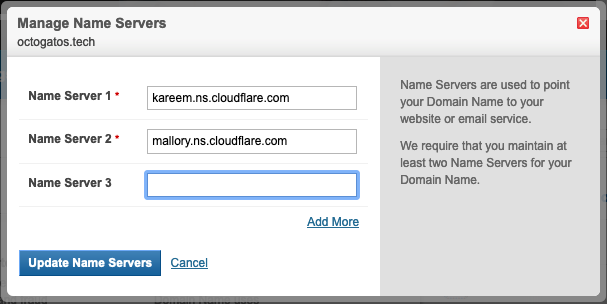
\includegraphics[width=0.7\textwidth]{DNS/nameServers}
  \caption{Configuraci\'on de los name servers para
           nuestro dominio.}
  \label{fig:nameServers}
\end{figure}

Se configuraron los siguiente registros DNS
externos en Cloudflare.
\begin{enumerate}
  \item A (Web Server - octogatos.tech - 52.87.39.6).

  \item A (Email Server - mail.octogatos.tech - 54.162.84.2).

  \item A (Email Server - postfixadmin.mail.octogatos.tech
                        - 54.162.84.2).

  \item AAAA (Web Server - octogatos.tech
                         - 2600:1f18:22c6:b16:1e05:b4d5:f19:61d).

  \item AAAA (Email Server - mail.octogatos.tech
                           - 2600:1f18:22c6:b00:9ca8:5c2a:c3c:d17f).

  \item CNAME (Web Server - www.octogatos.tech).

  \item MX (Web Server - 10 mail.octogatos.tech).

  \item TXT (Email Server - SPF).

  \item TXT (Email Server - DKIM).

  \item TXT (Email Server - DMARC).
\end{enumerate}
En la Figura \ref{fig:dnsExterno} se muestra la
evidencia respecto a esta configuraci\'on, misma
que puede ser verificada con el comando \ttt{dig},
salvo por aquellos registros para los que el proxy
de Cloudflare est\'a activo.
\begin{figure}[H]
  \centering
  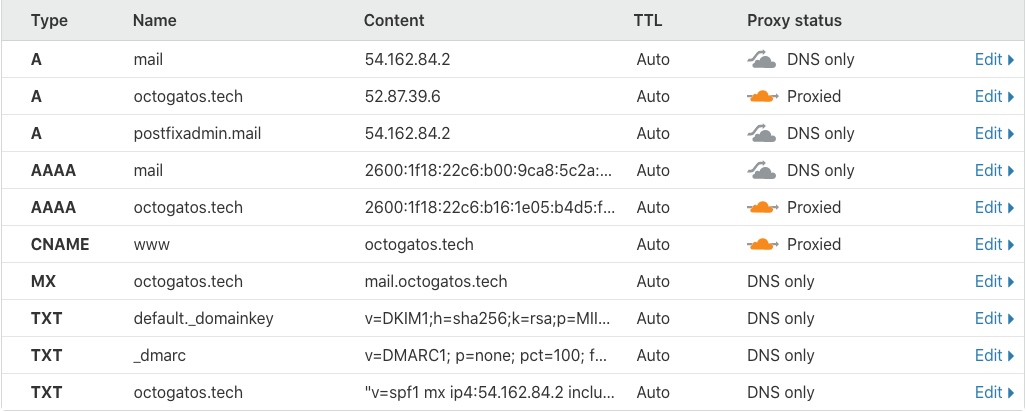
\includegraphics[width=0.85\textwidth]{DNS/dnsExterno}
  \caption{Configuraci\'on de los registros DNS externos.}
  \label{fig:dnsExterno}
\end{figure}

Adicionalmente, se configur\'o el registro PTR para
el servidor de correo, mediante la solicitud a Amazon
para abrir el puerto 25.

Se utiliz\'o Route 53 para configurar algunos registros
internos.   Para este fin, primero creamos una
``private hosted zone'', siguiendo las instrucciones
que aparecen en
\href{https://docs.aws.amazon.com/Route53/latest/DeveloperGuide/hosted-zone-private-creating.html}{esta liga} (recurso
de AWS).   Para crear esta zona, simplemente elegimos
la opci\'on ``Create hosted zone'', elegimos el
nombre de dominio ``octogatos.tech'', y la VPC en la
que estamos trabajando para asociar a nuestra nueva
zona. Una vez creada, es posible iniciar la configuraci\'on
de registros, que es semejante a la que se har\'ia
usualmente con un DNS externo, pero se utilizan las
direcciones IP privadas.   Un ejemplo de configuraci\'on
se puede ver en la Figura \ref{fig:defineRecord}, donde
el tipo de registro que se eligi\'o fue ``Simple'' (se
asocia el nombre de dominio con una \'unica direcci\'on
IP).

\begin{figure}[H]
  \centering
  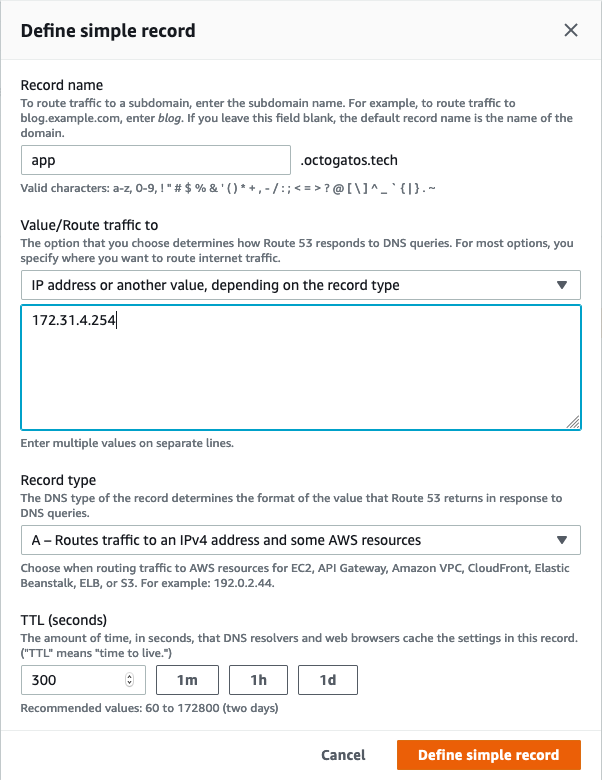
\includegraphics[width=0.44\textwidth]{DNS/defineRecord}
  \caption{Configuraci\'on del registro DNS interno para el
           app server usando Route 53.}
  \label{fig:defineRecord}
\end{figure}

Es posible configurar y crear m\'ultiples registros
a la vez, como se muestra en la Figura
\ref{fig:createRecord}

\begin{figure}[H]
  \centering
  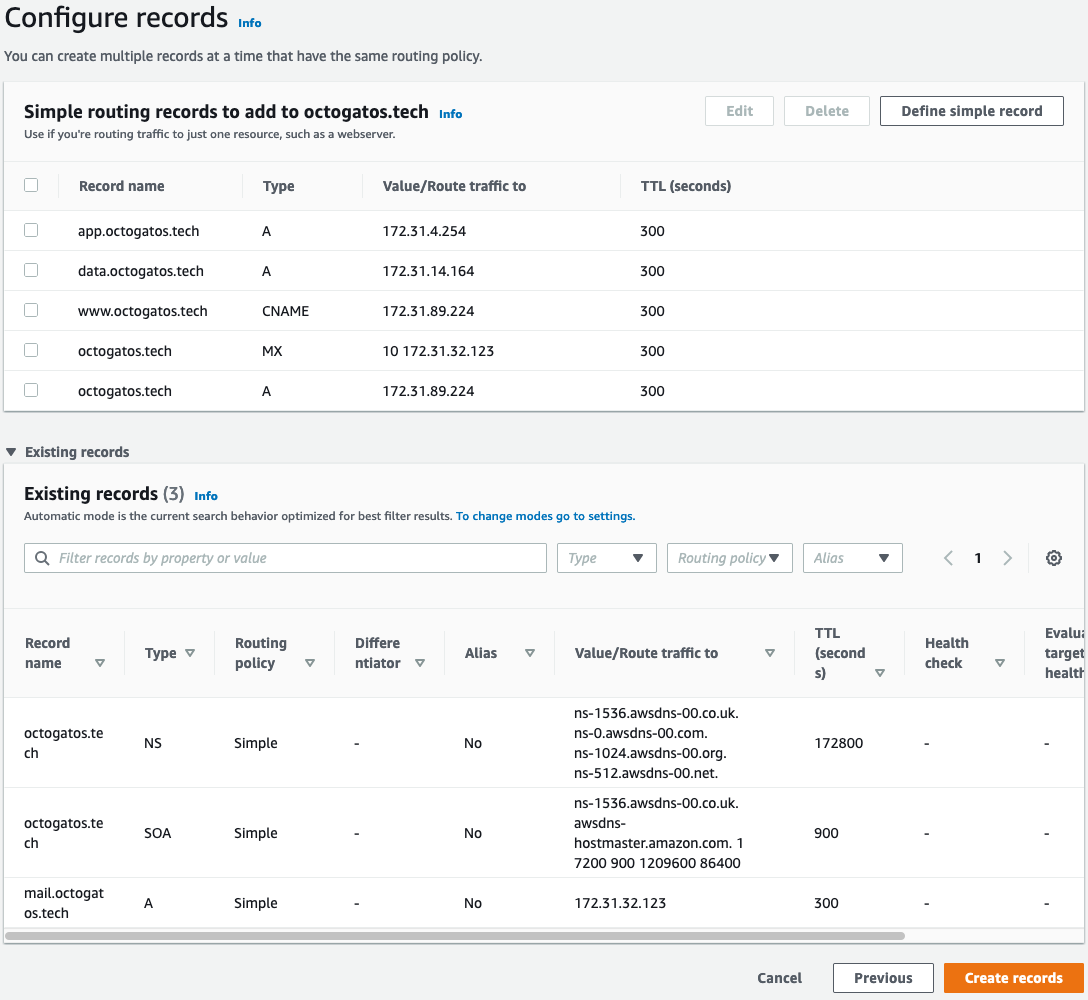
\includegraphics[width=0.8\textwidth]{DNS/createRecord}
  \caption{Creaci\'on de m\'ultiples registros DNS internos
           en Route 53.}
  \label{fig:createRecord}
\end{figure}


Usando Route 53, se configuraron los siguientes
registros.
\begin{enumerate}
  \item A (Web Server - octogatos.tech - 172.31.89.224).

  \item A (Email Server - mail.octogatos.tech - 172.31.32.123).

  \item A (App Server - 172.31.4.254).

  \item A (Data Server - 172.31.14.164).

  \item CNAME (Web Server - www.octogatos.tech).

  \item MX (Web Server - 10 172.31.32.123).
\end{enumerate}
La evidencia de esta configuraci\'on se muestra en
la Figura \ref{fig:createdRecord}
\begin{figure}[H]
  \centering
  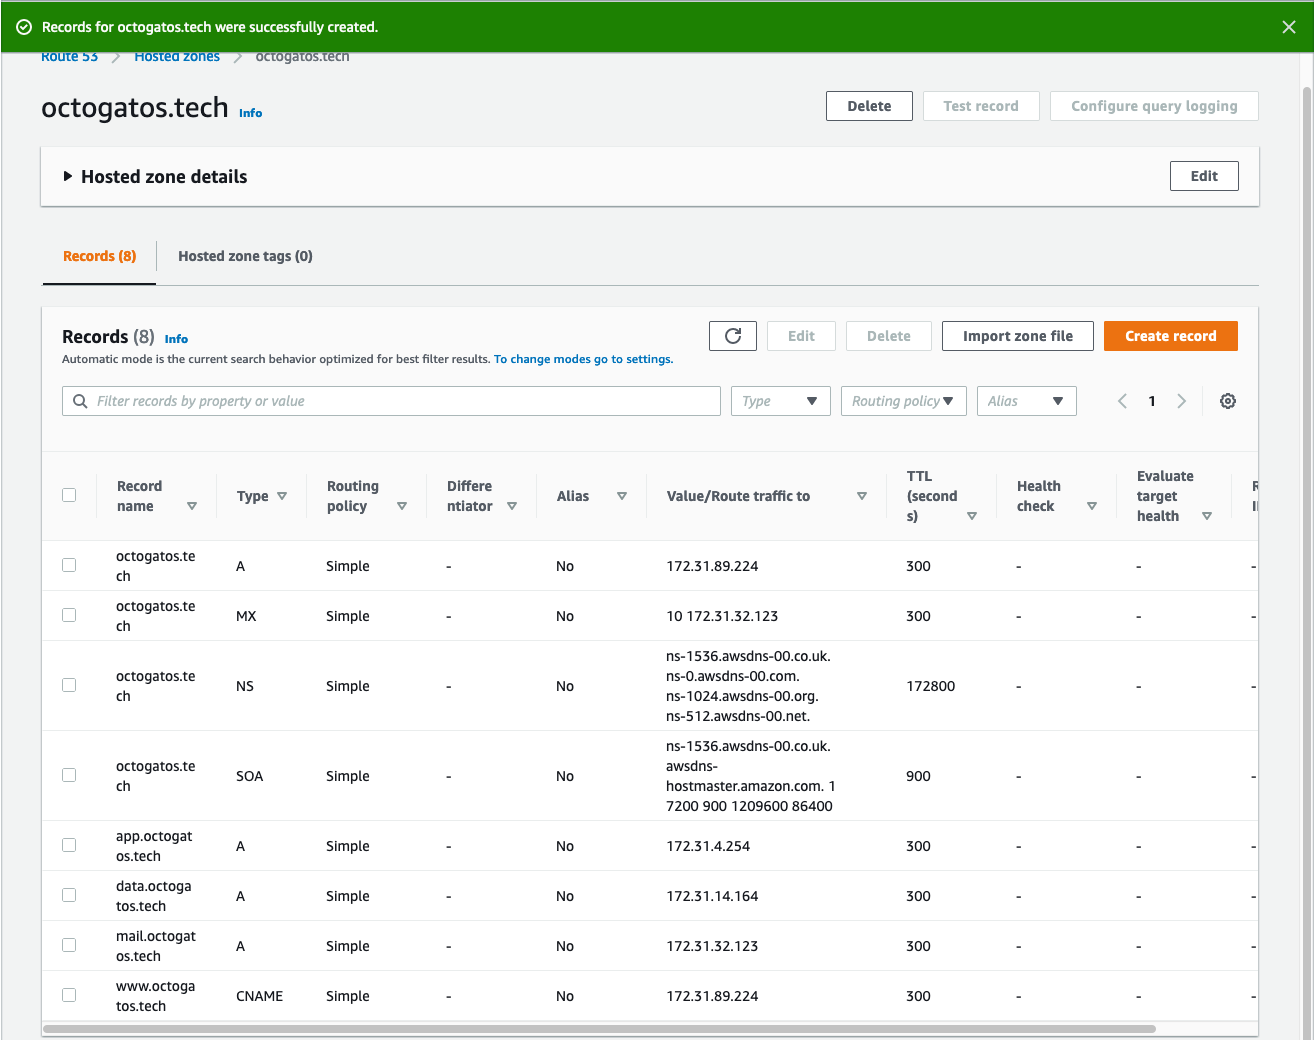
\includegraphics[width=0.8\textwidth]{DNS/createdRecord}
  \caption{Registros DNS internos configurados en Route 53.}
  \label{fig:createdRecord}
\end{figure}

%%%%%%%%%%%%%%%%%%%%%%%%%%%%%%%%%%%%%%%%%%%%%%%%%%%%%%%%%%%%%%%%
%%%%%%%%%%%%%%%%%%%%%%%%%%%%%%%%%%%%%%%%%%%%%%%%%%%%%%%%%%%%%%%%
%%%%%%%%%%%%%%%%%%%%%%%%%%%%%%%%%%%%%%%%%%%%%%%%%%%%%%%%%%%%%%%%
%%%%%%%%%%%%%%%%%%%%%%%%               %%%%%%%%%%%%%%%%%%%%%%%%%
%%%%%%%%%%%%%%%%%%%%%%%%%%%%%%%%%%%%%%%%%%%%%%%%%%%%%%%%%%%%%%%%
%%%%%%%%%%%%%%%%%%%%%%%%%%%%%%%%%%%%%%%%%%%%%%%%%%%%%%%%%%%%%%%%
%%%%%%%%%%%%%%%%%%%%%%%%%%%%%%%%%%%%%%%%%%%%%%%%%%%%%%%%%%%%%%%%

\section{Cloudflare}

Se utilaron tres servicios de
\href{https://www.cloudflare.com/}{Cloudflare}, a saber,
su DNS, como una capa de seguridad adicional entre el
usuario y el proxy de Cloudflare, y como Red de
Distribuci\'on de Contenidos (CDN).

Respecto a su uso como DNS, ya se habl\'o de la
configuraci\'on en la Secci\'on \ref{sec:dns}.   Para
su uso como CDN, configuramos dos reglas de CDN, una
para servir hojas de estilo (CSS) y otra para servir
im\'agenes.   Para la configuraci\'on simplemente
elegimos la regla de cach\'e y el recurso que queremos
que sea servido por Cloudflare.   En nuestro caso,
elegimos Edge Cache TTL, que nos permite indicar
un tiempo que, al transcurrir, Cloudflare solicitar\'a
una actualizaci\'on del recurso.   La configuraci\'on
de ambas reglas puede verse en la Figura
\ref{fig:pageRules}.

\begin{figure}[H]
  \centering
  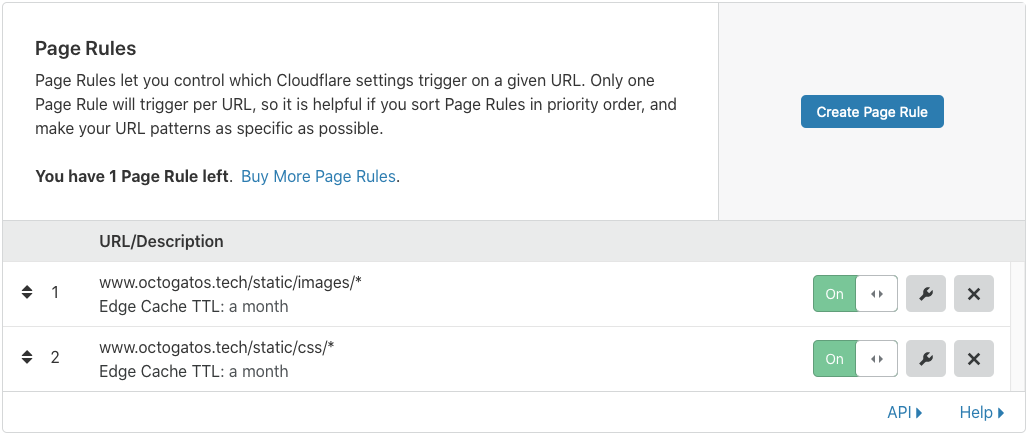
\includegraphics[width=0.8\textwidth]{cloudflare/pageRules}
  \caption{Configuraci\'on de page rules en Cloudflare.}
  \label{fig:pageRules}
\end{figure}

Para ver que estas reglas realmente est\'an funcionando,
podemos elegir la opci\'on ``Inspeccionar Elemento'' en
nuestra p\'agina \href{https://octogatos.tech}{octogatos.tech},
y notar que el valor \ttt{cf-cache-status} asociado a
a la imagen jazzCats.jpg es \ttt{HIT}, lo que significa que
fue encontrado al buscarse en el cache ofrecido por Cloudflare.
Puede notarse adem\'as que el valor de \ttt{server} es
cloudflare (Figura \ref{fig:pageRulesHit}).

% ALERT
% Actualizar el SS por uno que no tenga un 404

\begin{figure}[H]
  \centering
  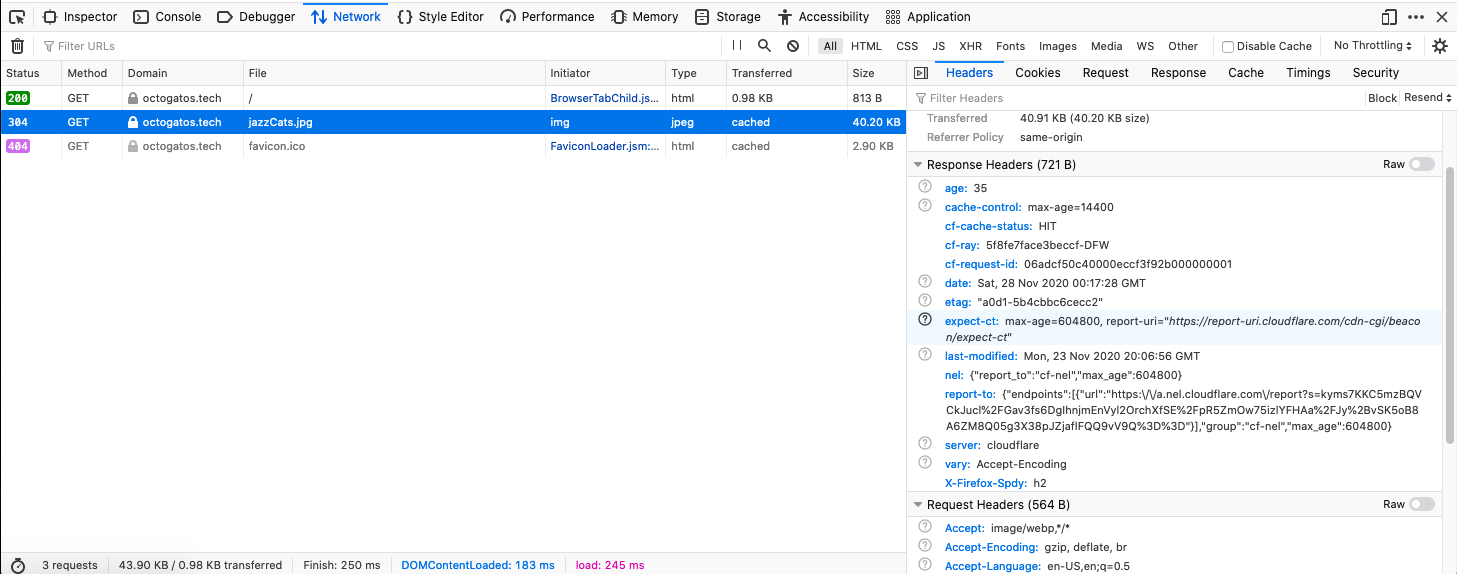
\includegraphics[width=\textwidth]{cloudflare/pageRulesHit}
  \caption{Configuraci\'on de page rules en Cloudflare.}
  \label{fig:pageRulesHit}
\end{figure}

Por otro lado, el modo de encriptaci\'on que se
configur\'o en Cloudflare es Completo (estricto).
Como ya se mencion\'o, Cloudflare ofrece la
encriptaci\'on entre el usuario final y sus
servidores (que estamos usando como proxies),
y nuestros certificados de Let's Encrypt proporcionan
la seguridad entre los servidores de Cloudflare
y nuestro servidor en AWS.   El estado actual de
la configuraci\'on de SSL/TLS puede verse en la
Figura \ref{fig:cfEncryption}.

\begin{figure}[H]
  \centering
  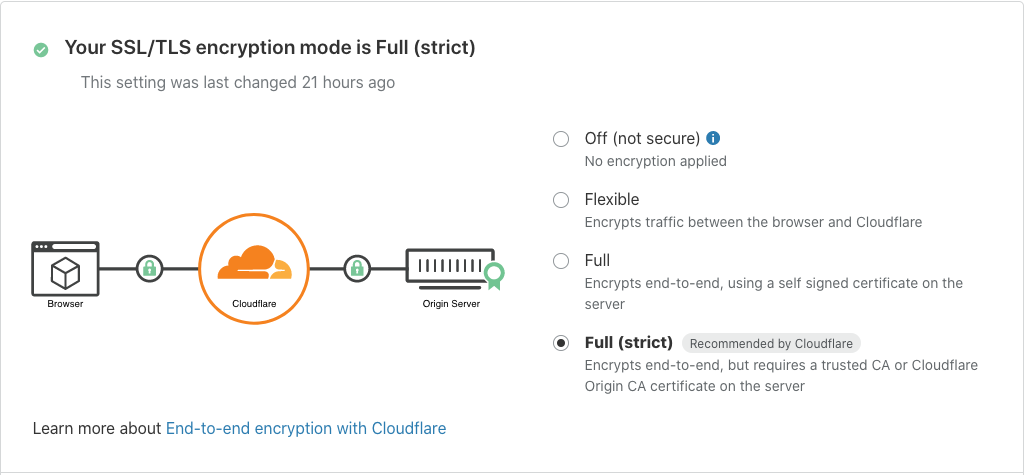
\includegraphics[width=\textwidth]{cloudflare/cfEncryption}
  \caption{Configuraci\'on de SSL/TLS en Cloudflare.}
  \label{fig:cfEncryption}
\end{figure}


%%%%%%%%%%%%%%%%%%%%%%%%%%%%%%%%%%%%%%%%%%%%%%%%%%%%%%%%%%%%%%%%
%%%%%%%%%%%%%%%%%%%%%%%%%%%%%%%%%%%%%%%%%%%%%%%%%%%%%%%%%%%%%%%%
%%%%%%%%%%%%%%%%%%%%%%%%%%%%%%%%%%%%%%%%%%%%%%%%%%%%%%%%%%%%%%%%
%%%%%%%%%%%%%%%%%%%%%%%%               %%%%%%%%%%%%%%%%%%%%%%%%%
%%%%%%%%%%%%%%%%%%%%%%%%%%%%%%%%%%%%%%%%%%%%%%%%%%%%%%%%%%%%%%%%
%%%%%%%%%%%%%%%%%%%%%%%%%%%%%%%%%%%%%%%%%%%%%%%%%%%%%%%%%%%%%%%%
%%%%%%%%%%%%%%%%%%%%%%%%%%%%%%%%%%%%%%%%%%%%%%%%%%%%%%%%%%%%%%%%

\section{Web Server}

Para nuestro Web Server utilizamos la instancia EC2 que
fue creada en la Pr\'actica 2, por lo que no ahondaremos
en detalles respecto a su creaci\'on.   Es importante
recalcar que tambi\'en reutilizamos el certificado
expedido por \href{https://letsencrypt.org/}{Let's Encrypt},
y configurado con \href{https://certbot.eff.org/}{Certbot},
as\'i como la direcci\'on IP el\'astica de la Pr\'actica 2,
por lo que la configuraci\'on de la instancia en AWS se ve
como en la Figura \ref{fig:web-instancia}.

\begin{figure}[H]
  \centering
  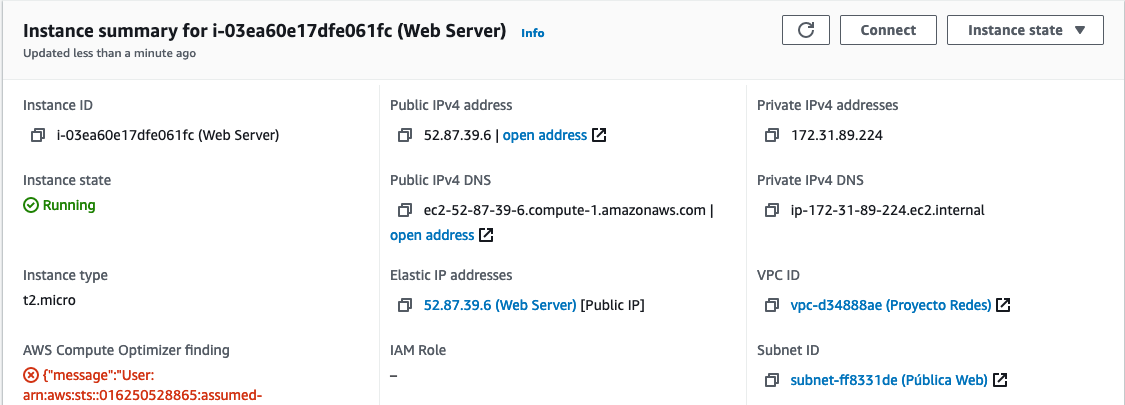
\includegraphics[width=\textwidth]{web/instancia}
  \caption{Configuraci\'on de la instancia del Web Server
           en AWS.}
  \label{fig:web-instancia}
\end{figure}

Como se puede ver en la figura, esta instancia se
encuentra en una subred, identificada con el nombre
``P\'ublica Web'', cuya configuraci\'on se muestra
en la figura \ref{fig:web-subred}.

\begin{figure}[H]
  \centering
  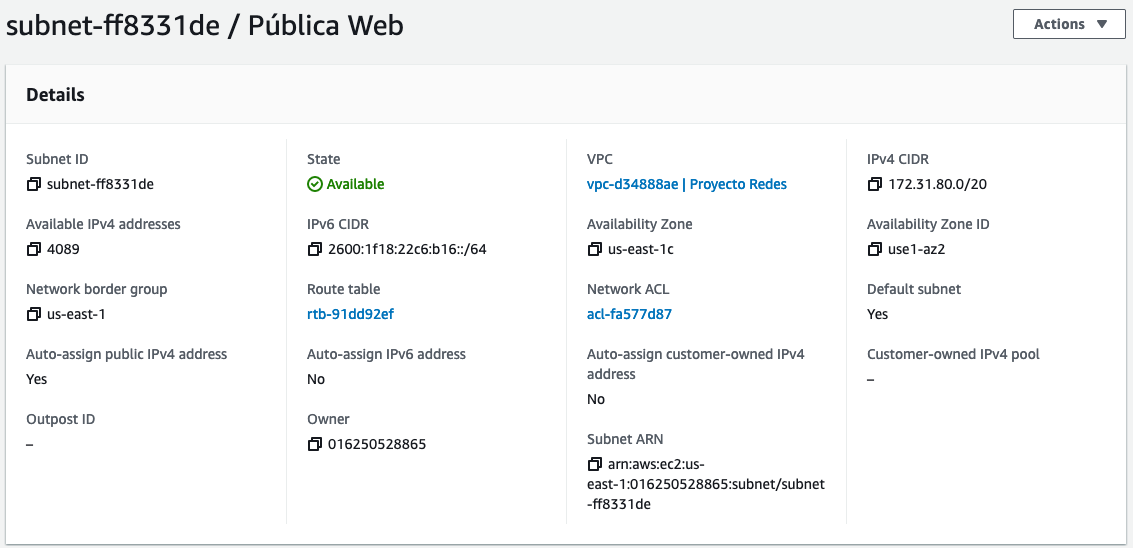
\includegraphics[width=\textwidth]{web/subred}
  \caption{Configuraci\'on de la primera subred p\'ublica.}
  \label{fig:web-subred}
\end{figure}

Adem\'as, esta instancia cuenta con una direcci\'on IPv6,
misma que puede verse en la configuraci\'on de red de la
instancia, misma que puede apreciarse en la Figura
\ref{fig:web-ipv6}.   N\'otese que la direcci\'on IPv6
de esta instancia efectivamente coincide con la que se
asign\'o a la subred correspondiente.

\begin{figure}[H]
  \centering
  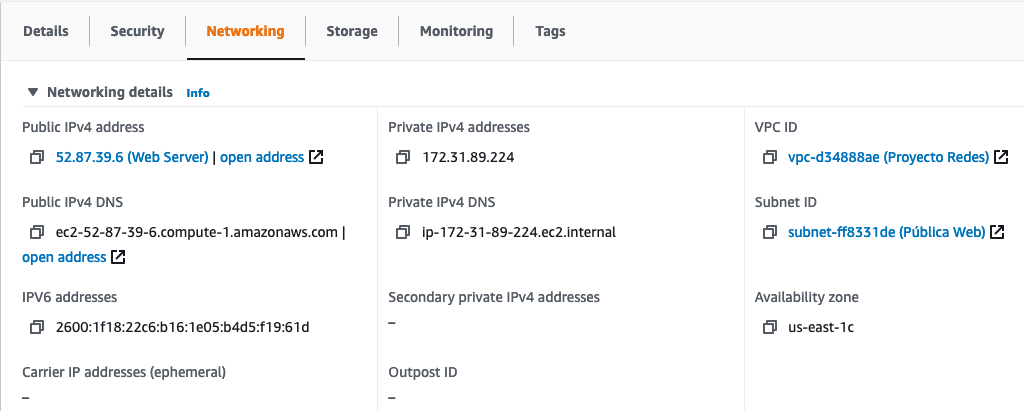
\includegraphics[width=\textwidth]{web/ipv6}
  \caption{Configuraci\'on de red del servidor web.}
  \label{fig:web-ipv6}
\end{figure}

Nuestro servidor web act\'ua principalmente como
forward y reverse proxy.   Esta opci\'on se habilita
como parte de la configuraci\'on del servidor Apache.
Hay varios recursos en internet sobre c\'omo realizar
esta configuraci\'on paso a paso, por ejemplo, es
posible seguir las instrucciones dadas por
\href{https://www.digitalocean.com/community/tutorials/how-to-use-apache-http-server-as-reverse-proxy-using-mod_proxy-extension}{este
tutorial} de Digital Ocean.   Para llevar a cabo,
la configuraci\'on, primero es necesario activar
algunos m\'odulos de apache, lo que puede hacerse
con los comandos
\begin{lstlisting}
$ sudo a2enmod proxy
$ sudo a2enmod proxy_http
$ sudo a2enmod rewrite
$ sudo a2enmos proxy_connect
$ sudo a2enmod proxy_html
\end{lstlisting}

Existe la posibilidad de que el m\'odulo no est\'e
instalado, en cuyo caso puede instalarse con el
comando
\begin{lstlisting}
sudo apt install -y libapache2-mod-proxy-html libxml2-dev
\end{lstlisting}

Una vez habilitados estos m\'odulos, procedemos
a actualizar la configuraci\'on del servidor
Apache, con el comando
\begin{lstlisting}
sudo vi /etc/apache2/sites-available/redesfc.conf
\end{lstlisting}

Tambi\'en es necesario actualizar la configuraci\'on
creada por Certbot cuando obtuvimos el certificado
de Let's Encrypt, para el virtual host de HTTPS en
el puerto 443, lo que puede hacerse con el siguiente
comando
\begin{lstlisting}
sudo vi /etc/apache2/sites-available/redesfc-le-ssl.conf
\end{lstlisting}

Las configuraciones deben de verse como en la
Figura \ref{fig:web-mapache}.
\begin{figure}[H]
  \centering
  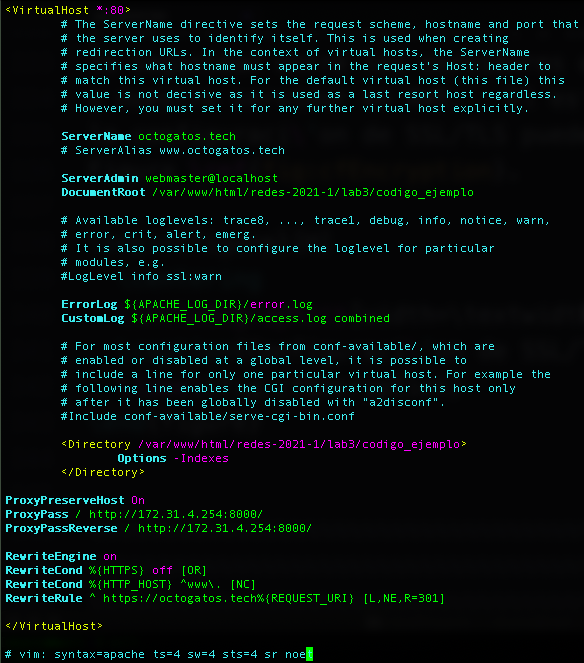
\includegraphics[width=0.45\textwidth]{web/mapache80}
  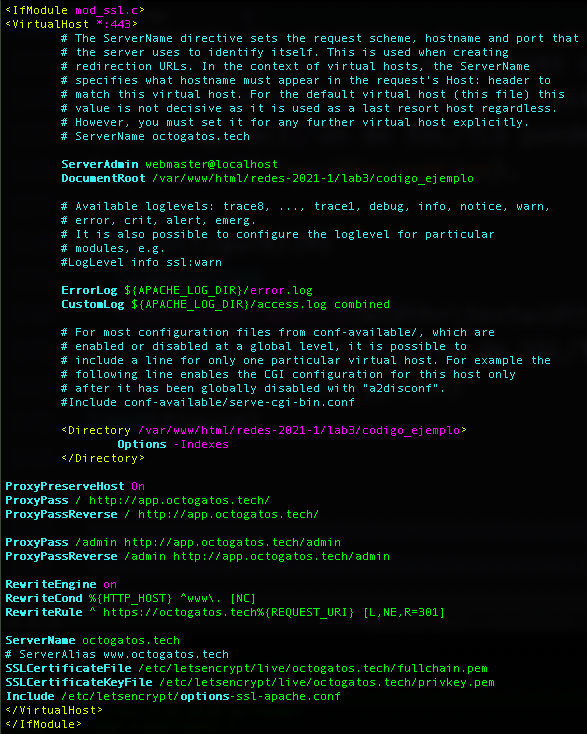
\includegraphics[width=0.45\textwidth]{web/mapache443}
  \caption{Configuraci\'on del servidor Apache como proxy.}
  \label{fig:web-mapache}
\end{figure}

Las l\'ineas que nos interesan son aquellas que empiezan
con la palabra ``Proxy'', en donde se activa la opci\'on
\ttt{ProxyPreserveHost}, que indica a Apache que debe
mantener la direcci\'on url del host que actua como proxy,
y las opciones \ttt{ProxyPass} y \ttt{ProxyReverse}, que
indican a Apache que redireccione las peticiones hacia y
desde el servidor al que est\'a sirviendo como proxy (en
nuestro caso, el servidor de aplicaci\'on).

En las misma figura es posible notar que tenemos
la l\'inea \ttt{Options -Indexes}, que deshabilita
la opci\'on de enlistar los contenidos de las carpetas
que se encuentran en nuestro directorio ra\'iz.

Adicionalmente, y tambi\'en en la Figura \ref{fig:web-mapache},
es posible encontrar algunas l\'ineas que empiezan con
la palabra ``Rewrite''.   La finalidad de estas es lograr
la redirecci\'on de
\href{http://octogatos.tech}{http://octogatos.tech},
\href{http://www.octogatos.tech}{http://www.octogatos.tech}, y
\href{https://www.octogatos.tech}{https://www.octogatos.tech}
a \href{https://octogatos.tech}{https://octogatos.tech}.


%%%%%%%%%%%%%%%%%%%%%%%%%%%%%%%%%%%%%%%%%%%%%%%%%%%%%%%%%%%%%%%%
%%%%%%%%%%%%%%%%%%%%%%%%%%%%%%%%%%%%%%%%%%%%%%%%%%%%%%%%%%%%%%%%
%%%%%%%%%%%%%%%%%%%%%%%%%%%%%%%%%%%%%%%%%%%%%%%%%%%%%%%%%%%%%%%%
%%%%%%%%%%%%%%%%%%%%%%%%               %%%%%%%%%%%%%%%%%%%%%%%%%
%%%%%%%%%%%%%%%%%%%%%%%%%%%%%%%%%%%%%%%%%%%%%%%%%%%%%%%%%%%%%%%%
%%%%%%%%%%%%%%%%%%%%%%%%%%%%%%%%%%%%%%%%%%%%%%%%%%%%%%%%%%%%%%%%
%%%%%%%%%%%%%%%%%%%%%%%%%%%%%%%%%%%%%%%%%%%%%%%%%%%%%%%%%%%%%%%%

\section{Configuraci\'on NAT}

Como se mencion\'o con anterioridad, con la finalidad
de ahorrar cr\'editos de AWS, configuramos una NAT
independiente de nuestro proyecto, \'unicamente con
dos subredes, una p\'ublica y una privada, cada una
con una instancia de EC2.   A continuaci\'on describimos
c\'omo se llev\'o a cabo dicha configuraci\'on; el punto
principal es que la instancia que corre en la subred
privada no tiene una direcci\'on IP p\'ublica, por lo
que no puede ser accedida desde el exterior de la VPC.
Para conectarnos a \'esta, utilizamos su direcci\'on
IP privada desde la instancia que se encuentra corriendo
en la subred p\'ublica.

Como prerrequisitos, consideramos que ya existe una
instancia corriendo (la que fue creada en la Pr\'actica
2), y que est\'a en la subred por omisi\'on, con la
VPC por omisi\'on, y la Route Table por omisi\'on.
La configuraci\'on de la subred por omisi\'on, que se
utilizar\'a como subred p\'ublica, se muestra en la
Figura \ref{fig:NAT-pubSubnet}.   Adem\'as de la
explicaci\'on brindada por el profesor en Discord,
nos apoyamos en el siguiente documento de AWS.
\href{https://docs.aws.amazon.com/vpc/latest/userguide/VPC_Scenario2.html}{https://docs.aws.amazon.com/vpc/latest/userguide/VPC\_Scenario2.html}

\begin{figure}[H]
  \centering
  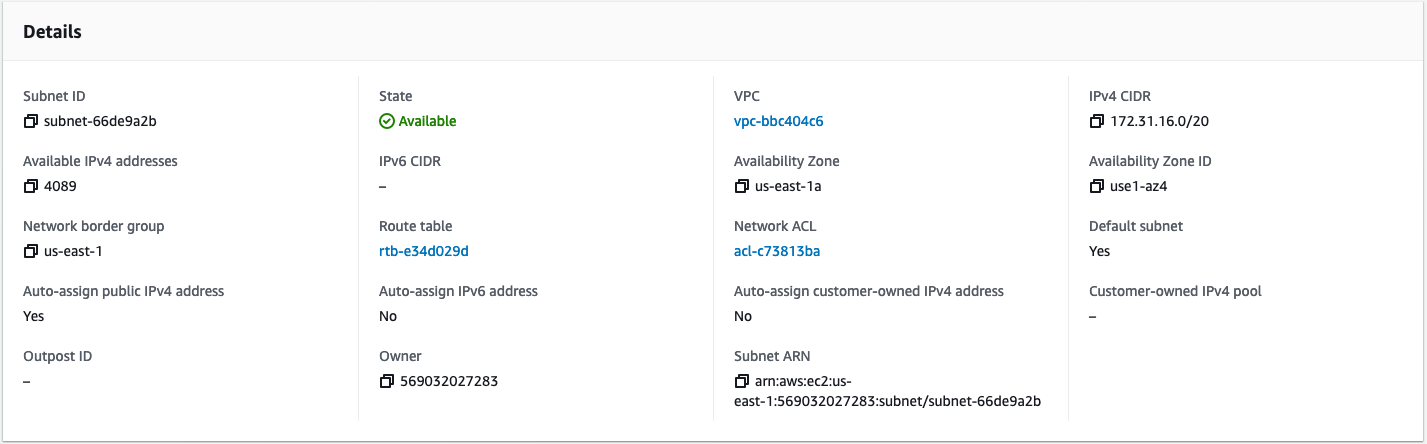
\includegraphics[width=\textwidth]{SSNAT/publicSubnet}
  \caption{Configuraci\'on de la subred p\'ublica.}
  \label{fig:NAT-pubSubnet}
\end{figure}

\begin{enumerate}
  \item Creamos una nueva subred, en la misma zona de
    disponibilidad que la red que ya ten\'iamos, y con
    conjunto de direcciones IPv4 en el mismo segmento
    que la anterior.   En la captura de pantalla hay un
    error, hab\'iamos nombrado ``P\'ublica'' a esta red,
    pero esta realmente es la privada (el error se
    corrigi\'o posteriormente).    La configuraci\'on
    puede verse en la Figura \ref{fig:NAT-priSubnet}. Una
    observaci\'on importante es que se deshabilit\'o
    la opci\'on de asignar autom\'aticamente una
    direcci\'on IPv4 a las instancias que se creen
    dentro de esta subred.   Adem\'as de la explicaci\'on
    compartida por el profesor, nos apoyamos en el
    siguiente documento de AWS: \href{https://docs.aws.amazon.com/cloudhsm/latest/userguide/create-subnets.html}{https://docs.aws.amazon.com/cloudhsm/latest/userguide/create-subnets.html}.
    \begin{figure}[H]
      \centering
      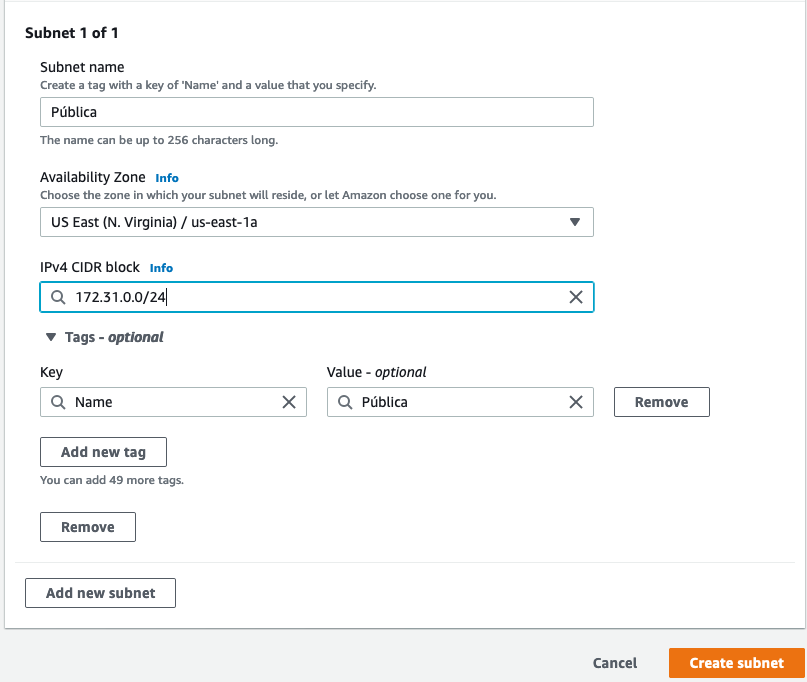
\includegraphics[width=0.8\textwidth]{SSNAT/privateSubnet}
      \caption{Configuraci\'on de la subred privada.}
      \label{fig:NAT-priSubnet}
    \end{figure}

  \item Posteriormente, creamos una nueva instancia,
    en la misma \'area de disponibilidad que la instancia
    anterior, pero en la subrede privada reci\'en creada.
    La configuraci\'on de esta instancia puede verse en
    la Figura \ref{fig:NAT-priInstance}.   Es importante hacer
    notar que esta instancia no cuenta con una direcci\'on
    IPv4.
    \begin{figure}[H]
      \centering
      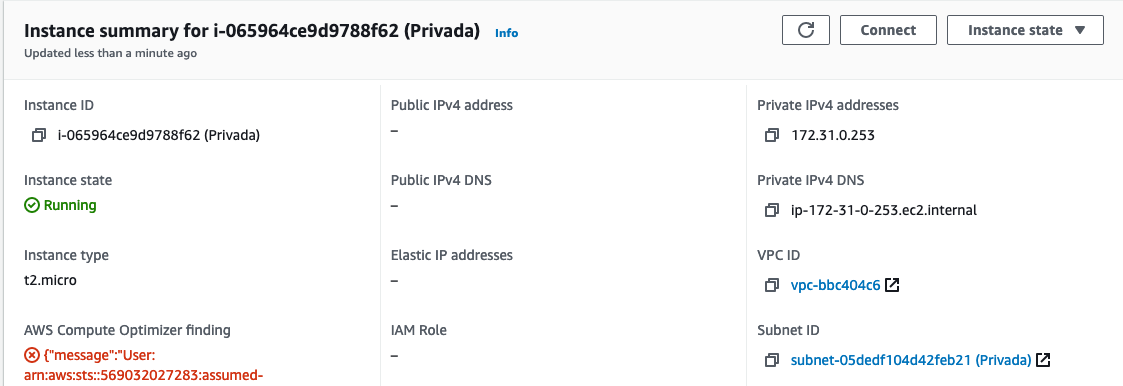
\includegraphics[width=\textwidth]{SSNAT/privateInstance}
      \caption{Configuraci\'on de la instancia privada.}
      \label{fig:NAT-priInstance}
    \end{figure}

  \item El siguiente paso fue crear el NAT gateway.   La
    configuraci\'on resultante aparece en la Figura
    \ref{fig:NAT-nat}.  Cabe resaltar la importancia de
    asignar una IP el\'astica al NAT gateway al momento
    de crearlo. Nos apoyamos en las instrucciones que el
    profesor comparti\'o en Discord y el siguiente
    documento de AWS:
    \href{https://aws.amazon.com/premiumsupport/knowledge-center/nat-gateway-vpc-private-subnet/}{https://aws.amazon.com/premiumsupport/knowledge-center/nat-gateway-vpc-private-subnet/}
    \begin{figure}[H]
      \centering
      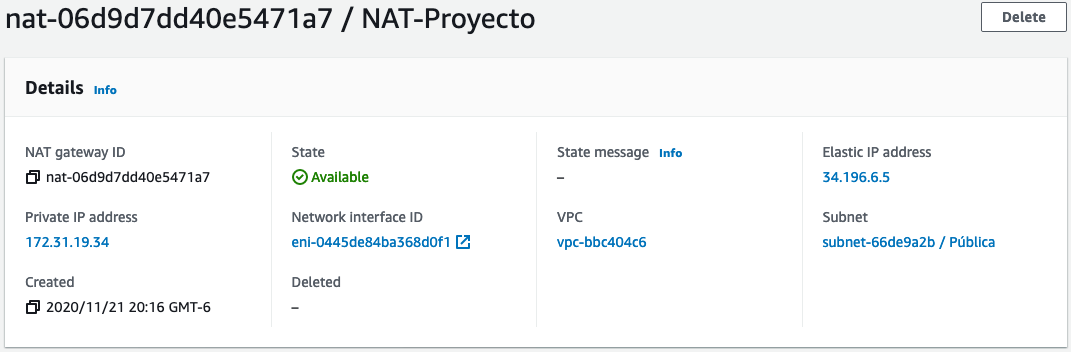
\includegraphics[width=\textwidth]{SSNAT/nat}
      \caption{Configuraci\'on del NAT gateway.}
      \label{fig:NAT-nat}
    \end{figure}

  \item Posteriormente, creamos una nueva tabla de
    ruteo.   Es necesario agregar una ruta, con destino
    \ttt{0.0.0.0/0} y target el NAT gateway reci\'en
    creado.   La configuraci\'on resultante puede
    verse en la Figura \ref{fig:NAT-routeTable}.
    \begin{figure}[H]
      \centering
      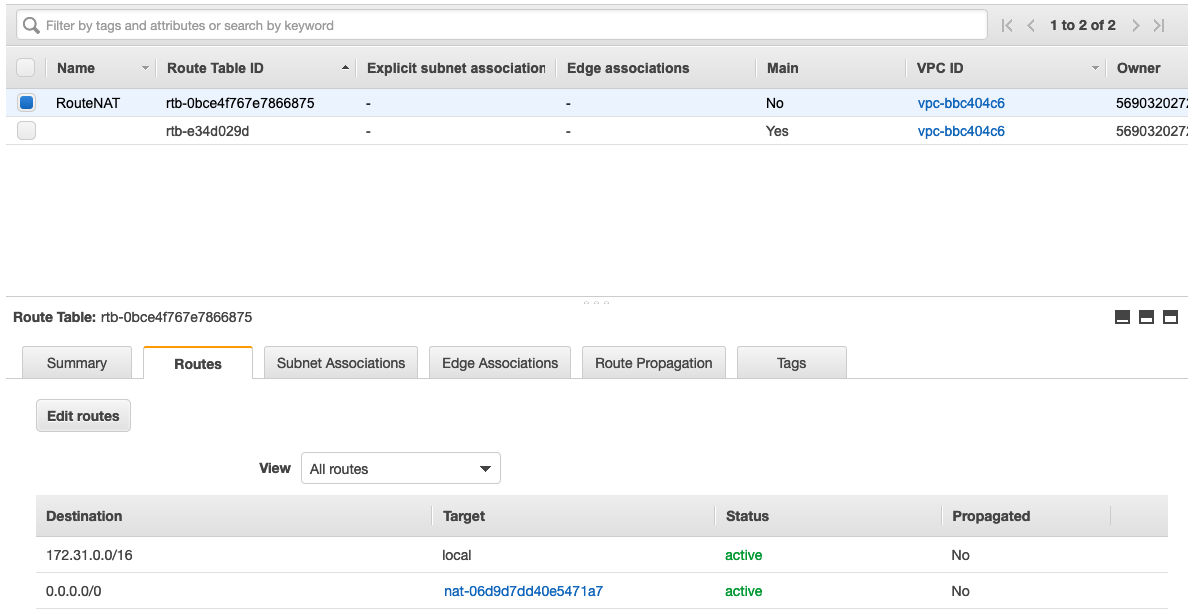
\includegraphics[width=\textwidth]{SSNAT/routeTable}
      \caption{Configuraci\'on de la nueva tabla de ruteo.}
      \label{fig:NAT-routeTable}
    \end{figure}

  \item Para terminar, asociamos la subred privada con
    la tabla de ruteo creada en el paso anterior. El
    resultado de esa asociaci\'on se observa en la Figura
    \ref{fig:subnetRouteTable}.
    \begin{figure}[H]
      \centering
      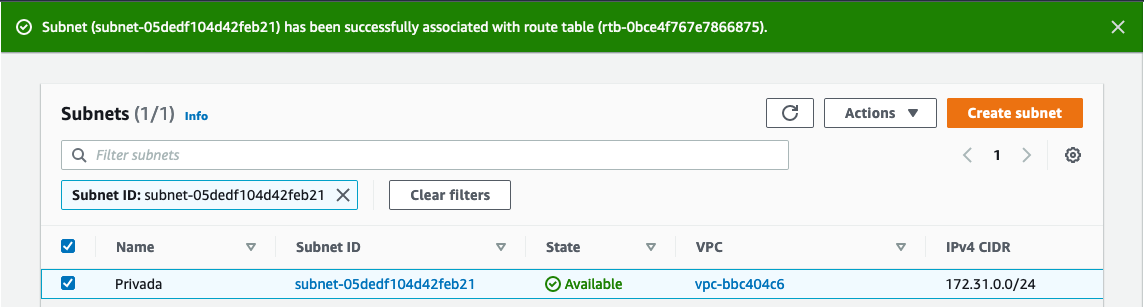
\includegraphics[width=\textwidth]{SSNAT/subnetRouteTable}
      \caption{Subred privada asociada a la nueva tabla
      de ruteo.}
      \label{fig:subnetRouteTable}
    \end{figure}
\end{enumerate}

Una vez terminada la configuraci\'on, podemos verificar
que funcione correctamente con los siguientes pasos.

\begin{enumerate}
  \item Ingresar a la instancia p\'ublica, con el
    comando
\begin{lstlisting}
$ ssh -i "practica2.pem" ubuntu@ec2-34-201-69-182.compute-1.amazonaws.com
\end{lstlisting}

  \item Una vez dentro de la instancia p\'ublica, ingresar
    a la privada mediante su direcci\'on IP privada, con
    el comando
\begin{lstlisting}
$ ssh -i "practica2.pem" ubuntu@172.31.0.253
\end{lstlisting}

  \item Verificar la conectividad a internet, por
    ejemplo, con un ping a google.com
\begin{lstlisting}
$ ping google.com
\end{lstlisting}

  \item Al no contar con direcci\'on IP p\'ublica
    ni siquiera es posible intentar conectarnos a
    la instancia privada externamente, pues su
    direcci\'on IP privada es relativa a la subred
    en la que est\'a.
\end{enumerate}

El resultado de los pasos antes descritos puede
revisarse en la Figura \ref{fig:NAT-result}.
\begin{figure}[H]
  \centering
  
\includegraphics[width=0.35\textwidth]{SSNAT/inception}
  \caption{It's like inception!}
\end{figure}

\begin{figure}[H]
  \centering
  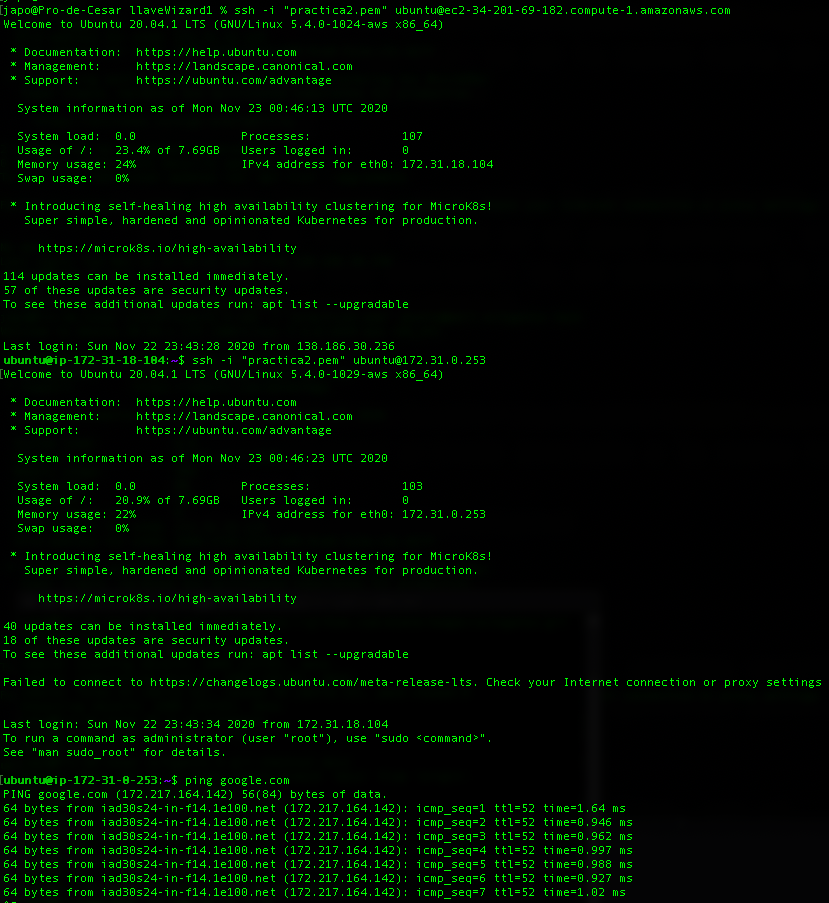
\includegraphics[width=\textwidth]{SSNAT/result}
  \caption{Subred privada asociada a la nueva tabla
  de ruteo.}
  \label{fig:NAT-result}
\end{figure}

\newpage

\section {Configuración del Data Server}

Para la configuración inicial del data server, lo primordial es tener
instalado y configurado el manejador de base de datos dentro de nuestro 
servidor. Para ello optamos por Postgres (12.5), el cual instalamos 
en nuestro servidos mediante los comandos:

\begin{lstlisting}
$ sudo apt install postgresql postgresql-contrib
\end{lstlisting}

\begin{figure}[H]
  \centering
  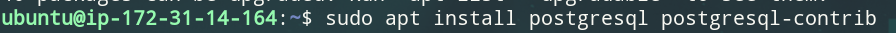
\includegraphics[width=\textwidth]{DATASERVER/exhibitA}
  \caption{Instalación de postgres en el data server.}
  \label{fig:DATASERVER-A}
\end{figure}

Como Postgres utiliza ``roles'' para manejar la autenticación y 
autorización de creación de base de datos, es necesario acceder 
al rol por omisión que crea Postgres para poder trabajar con su 
manejador de base de datos. Accedemos al usuario por medio de:

\begin{lstlisting}
$ sudo -i -u postgres
\end{lstlisting}

Y ahora podemos acceder sin problema alguno a Postgres:

\begin{figure}[H]
  \centering
  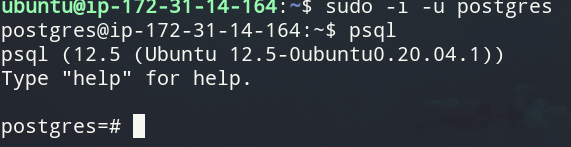
\includegraphics[width=\textwidth]{DATASERVER/exhibitB}
  \caption{Manejador de Base de Datos Postgresql.}
  \label{fig:DATASERVER-B}
\end{figure}

Y creamos nuestra base de datos \ttt{octogatos} que va a ser 
utilizada en este proyecto.

\begin{figure}[H]
  \centering
  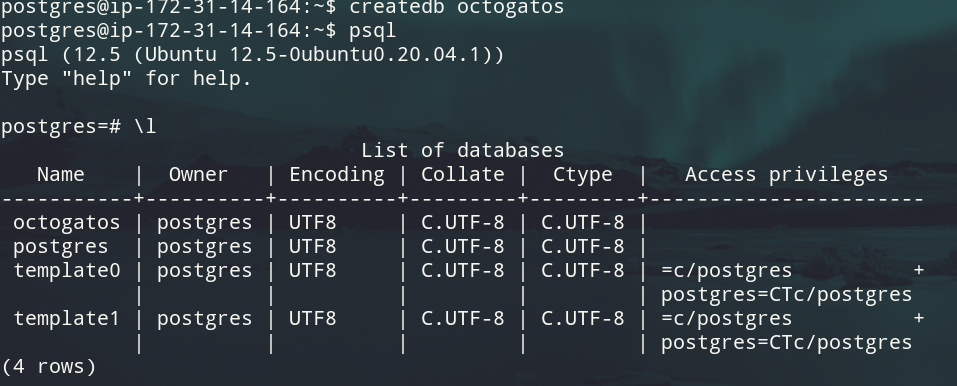
\includegraphics[width=\textwidth]{DATASERVER/exhibitC}
  \caption{Creación de la base de datos del proyecto.}
  \label{fig:DATASERVER-C}
\end{figure}

Como sólo se podrá conectar la App Server a este servidor, 
entonces es necesario indicar en la configuración que 
confíamos solo vamos a confiar en las conexiones locales 
(del mismo server a sí mismo) y en las conexiones que vengan
del App Server.

Para la conexión local, tenemos que modificar el archivo 
\ttt{pg\_hba.conf}, sustituyendo la línea:

\begin{lstlisting}
local   all             postgres                                peer
\end{lstlisting}

Por la línea:
\begin{lstlisting}
local   all             postgres                                trust
\end{lstlisting}

Reiniciamos nuestro servidor y listo, ya se pueden ejecutar 
\textit{scripts} de sql; por ejemplo creamos nuestra tabla 
``user'':

\begin{figure}[H]
  \centering
  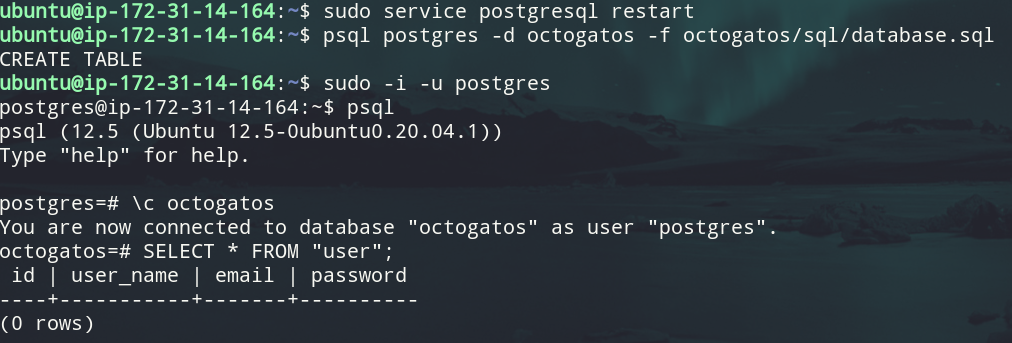
\includegraphics[width=\textwidth]{DATASERVER/exhibitE}
  \caption{Creación de la tabla usuarios.}
  \label{fig:DATASERVER-E}
\end{figure}

Para la conexión remota, primero tenemos que verificar a qué 
dirección IP se encuentra ligada el puerto 5432 (el puerto 
que usa Postgres).

\begin{figure}[H]
  \centering
  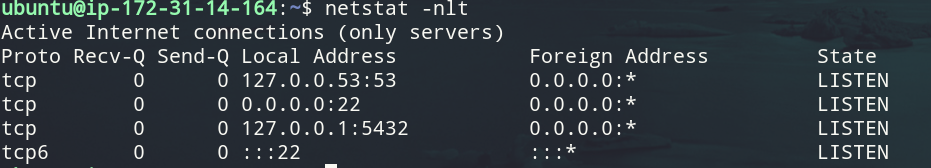
\includegraphics[width=\textwidth]{DATASERVER/exhibitF}
  \caption{La dirección del puerto 5432.}
  \label{fig:DATASERVER-E}
\end{figure}

Si nosotros tratamos de conectarnos a este puerto, entonces no 
vamos a tener éxito:

\begin{figure}[H]
  \centering
  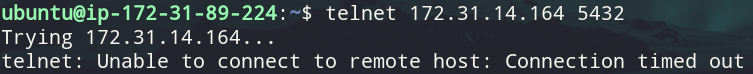
\includegraphics[width=\textwidth]{DATASERVER/exhibitG}
  \caption{Primero intento de conexión al puerto 5432.}
  \label{fig:DATASERVER-G}
\end{figure}

Para poder resolver esto, necesitamos configurar nuestros 
archivos \ttt{postgresql.conf} y \ttt{pg\_hba.conf}. 
En el primer archivo cambiamos el valor de 
\ttt{listen\_addresses} por:

\begin{lstlisting}
listen_addresses = '*'
\end{lstlisting}

Y también agregamos la dirección IP privada de la App
Server  al segundo archivo:
\begin{lstlisting}
host    all             all              172.31.4.254/0                       trust
\end{lstlisting}

\begin{figure}[H]
  \centering
  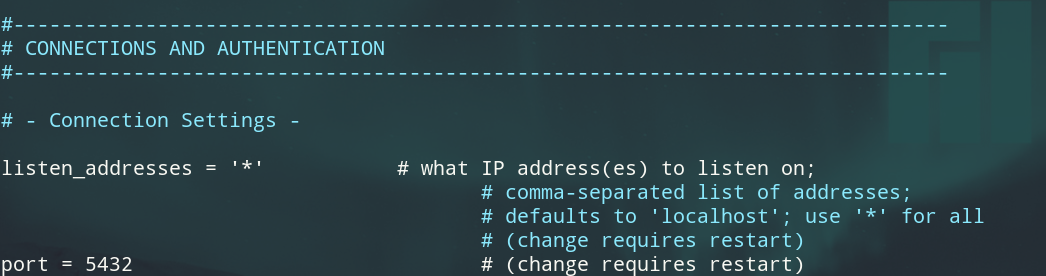
\includegraphics[width=\textwidth]{DATASERVER/exhibitI}
  \label{fig:DATASERVER-I}
\end{figure}

\begin{figure}[H]
  \centering
  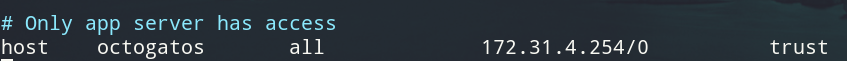
\includegraphics[width=\textwidth]{DATASERVER/exhibitJ}
  \label{fig:DATASERVER-J}
\end{figure}

Sin embargo, si lo dejamos como lo tenemos ahorita, nuestro 
servidor va a aceptar las conexiones de cualquier servidor,
por lo tanto tenemos que agregar este tipo de restricción 
al \textit{security groups} de nuestro servidor.

\begin{figure}[H]
  \centering
  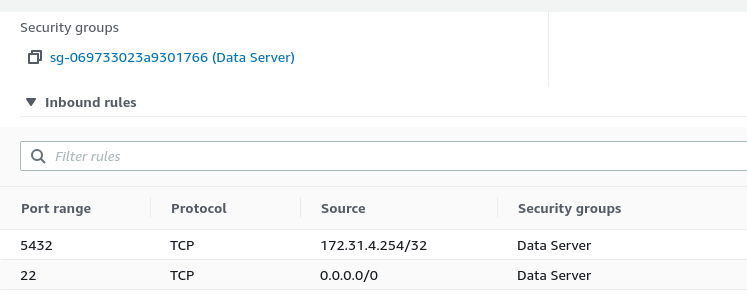
\includegraphics[width=\textwidth]{DATASERVER/exhibitK}
  \label{fig:DATASERVER-K}
\end{figure}

Y listo, si accedemos a nuestro App Server y tratamos de 
conectar a postgres, entonces vamos a tener éxito. Mientras
que si nos conectamos desde cualquier otro servidor o 
dispositivo dentro de la red, entonces no se va a aceptar la 
conexión.

\begin{figure}[H]
  \centering
  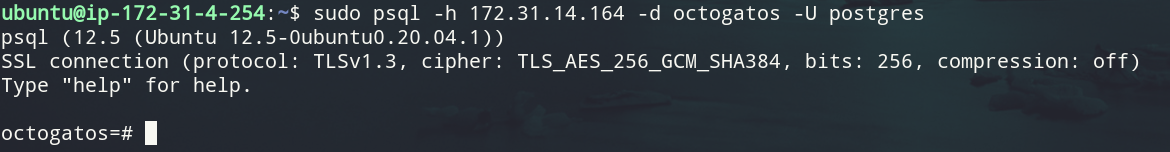
\includegraphics[width=\textwidth]{DATASERVER/exhibitL}
  \caption{Intento exitoso para conectarse al Data Server desde la App Server.}
  \label{fig:DATASERVER-L}
\end{figure}

\end{document}
